% Generated by jats2tex@0.11.1.0
\documentclass{article}
\usepackage[T1]{fontenc}
\usepackage[utf8]{inputenc} %% *
\usepackage[portuges,spanish,english,german,italian,russian]{babel} %% *
\usepackage{amstext}
\usepackage{authblk}
\usepackage{unicode-math}
\usepackage{multirow}
\usepackage{graphicx}
\usepackage{etoolbox}
\usepackage{xtab}
\usepackage{enumerate}
\usepackage{hyperref}
\usepackage{penalidades}
\usepackage[footnotesize,bf,hang]{caption}
\usepackage[nodayofweek,level]{datetime}
\setmainfont{Linux Libertine O}
\renewcommand*{\thefootnote}{\alph{footnote}}
\makeatletter
\newcommand{\fn}{\afterassignment\fn@aux\count0=}
\newcommand{\fn@aux}{\csname fn\the\count0\endcsname}
\makeatother

\newcommand{\journalid}{Cien Saude Colet}
\newcommand{\journaltitle}{Ciência \& Saúde Coletiva}
\newcommand{\abbrevjournaltitle}{Ciênc. saúde coletiva}
\newcommand{\issnppub}{1413-8123}
\newcommand{\issnepub}{1678-4561}
\newcommand{\publishername}{\textsc{abrasco} - Associação Brasileira de Saúde Coletiva}
\newcommand\publisherid{S1413-81232014000100026}
\newcommand\articleid{\textsc{doi} 10.1590/1413-81232014191.2007}
\def\subject{Article}\newcommand{\subtitlestyle}[1]{-- \emph{#1}\medskip}
\newcommand{\transtitlestyle}[1]{\par\medskip\Large #1}
\newcommand{\transsubtitlestyle}[1]{-- \Large\emph{ #1}}

\newcommand{\titlegroup}{
\ifdef{\subtitle}{\subtitlestyle{\subtitle}}{}
\ifdef{\transtitle}{\transtitlestyle{\transtitle}}{}
\ifdef{\transsubtitle}{\transsubtitlestyle{\transsubtitle}}{}
}

\title{Fatores que influenciam a adoção de ferramentas de \textsc{tic} nos experimentos
de bioinformática de organizações biofarmacêuticas\titlegroup{}}
\newcommand{\subtitle}{um estudo de caso no Instituto Nacional do Câncer}
\newcommand{\transtitle}{Factors affecting the adoption of \textsc{ict} tools in
experiments with bioinformatics in biopharmaceutical organizations}
\newcommand{\transsubtitle}{a case study in the Brazilian Cancer Institute}
\author{Pitassi, Claudio}
\author{Gonçalves, Antonio Augusto}
\author{Moreno, Valter de Assis}
\affil{Universidade Estácio de Sá}
\affil{Instituto Nacional do Câncer}
\affil{Faculdades Ibmec}
\date{ 01 2014}
\def\volume{19}
\def\issue{01}
\def\fpage{257}
\def\lpage{268}
\def\permissions{All the contents of this journal, except where otherwise noted,
is licensed under a Creative Commons Attribution License}
\newcommand{\kwdgroup}{\textsc{tic}, Inovação tecnológica, Biologia molecular,
Bioinformática, Biofarmacêutica}
\newcommand{\kwdgroupen}{\textsc{ict}, Technological innovation, Molecular biology,
Bioinformatics, Biopharmaceuticals}

\begin{document}
\selectlanguage{portuges}
\section*{Metadados não aplicados}
\begin{itemize}
\item[\textbf{língua do artigo}]{Português}
\ifdef{\journalid}{\item[\textbf{journalid}] \journalid}{}
\ifdef{\journaltitle}{\item[\textbf{journaltitle}] \journaltitle}{}

\ifdef{\journalsubtitle}{\item[\textbf{journalsubtitle}] \journaltitle}{}
\ifdef{\transjournaltitle}{\item[\textbf{journaltitle}] \journaltitle}{}
\ifdef{\transjournalsubtitle}{\item[\textbf{journalsubtitle}] \journaltitle}{}

\ifdef{\abbrevjournaltitle}{\item[\textbf{abbrevjournaltitle}]
\abbrevjournaltitle}{}
\ifdef{\issnppub}{\item[\textbf{issnppub}] \issnppub}{}
\ifdef{\issnepub}{\item[\textbf{issnepub}] \issnepub}{}
\ifdef{\publishername}{\item[\textbf{publishername}] \publishername}{}
\ifdef{\publisherid}{\item[\textbf{publisherid}] \publisherid}{}
\ifdef{\subject}{\item[\textbf{subject}] \subject}{}
\ifdef{\transtitle}{\item[\textbf{transtitle}] \transtitle}{}
\ifdef{\authornotes}{\item[\textbf{authornotes}] \authornotes}{}
\ifdef{\articleid}{\item[\textbf{articleid}] \articleid}{}
\ifdef{\volume}{\item[\textbf{volume}] \volume}{}
\ifdef{\issue}{\item[\textbf{issue}] \issue}{}
\ifdef{\fpage}{\item[\textbf{fpage}] \fpage}{}
\ifdef{\lpage}{\item[\textbf{lpage}] \lpage}{}
\ifdef{\permissions}{\item[\textbf{permissions}] \permissions}{}
\end{itemize}
\maketitle

\begingroup

\begin{abstract}

O objetivo deste artigo é identificar e analisar os fatores que influenciaram a
adoção de ferramentas de Tecnologias de Informação e de Comunicação (\textsc{tic}) nos
experimentos de Bioinformática do Instituto Nacional do Câncer (Inca). Trata-se
de um estudo de campo único descritivo e exploratório, dentro da tradição
qualitativa. As evidências foram coletadas principalmente em entrevistas de
fundo com os gestores de áreas da Coordenação Geral Técnico-Científica e da
Divisão de Tecnologia da Informação do Inca. As respostas foram tratadas pelo
método de análise de conteúdo do tipo categorial. As categorias de análise foram
definidas a partir da revisão da literatura e consolidadas nos sete fatores do
Modelo Tecnologia-Organização-Ambiente (\textsc{toe}) adaptado para este estudo. O modelo
proposto permitiu demonstrar como atuam no caso do Inca os fatores que impactam
a adoção das complexas \textsc{tic} usadas nos experimentos de Bioinformática,
contribuindo para investigações em duas áreas de importância crescente para o
Complexo Econômico-Industrial de Saúde brasileiro: a inovação tecnológica e a
Biotecnologia. Com base nas evidências coletadas, uma questão é formulada: em
que medida o alinhamento dos fatores pertinentes à adoção das \textsc{tic} nos
experimentos de Bioinformática pode aumentar a capacidade de inovar de uma
organização biofarmacêutica brasileira?

\iflanguage{portuges}{\medskip\noindent\textbf{Palavras-chave:} \kwdgroup}{}
\iflanguage{english}{\medskip\noindent\textbf{Keywords:} \kwdgroupen}{}
\iflanguage{spanish}{\medskip\noindent\textbf{Palavras claves:} \kwdgroupes}{}
\iflanguage{french}{\medskip\noindent\textbf{Mots clés:} \kwdgroupfr}{}
\end{abstract}
\endgroup

\begingroup
\renewcommand{\section}[1]{\subsection*{#1}}
\begin{otherlanguage}{english}

\begin{abstract}

The scope of this article is to identify and analyze the factors that influence
the adoption of \textsc{ict} tools in experiments with bioinformatics at the Brazilian
Cancer Institute (\textsc{inca}). It involves a descriptive and exploratory qualitative
field study. Evidence was collected mainly based on in-depth interviews with the
management team at the Research Center and the \textsc{it} Division. The answers were
analyzed using the categorical content method. The categories were selected from
the scientific literature and consolidated in the
Technology-Organization-Environment (\textsc{toe}) framework created for this study. The
model proposed made it possible to demonstrate how the factors selected impacted
\textsc{inca}´s adoption of bioinformatics systems and tools, contributing to the
investigation of two critical areas for the development of the health industry
in Brazil, namely technological innovation and bioinformatics. Based on the
evidence collected, a research question was posed: to what extent can the
alignment of the factors related to the adoption of \textsc{ict} tools in experiments
with bioinformatics increase the innovation capacity of a Brazilian
biopharmaceutical organization?

\ifdef{\kwdgroupen}{\medskip\noindent\textbf{Keywords:} \kwdgroupen}{}
\end{abstract}

\end{otherlanguage}

\endgroup

\begin{figure}
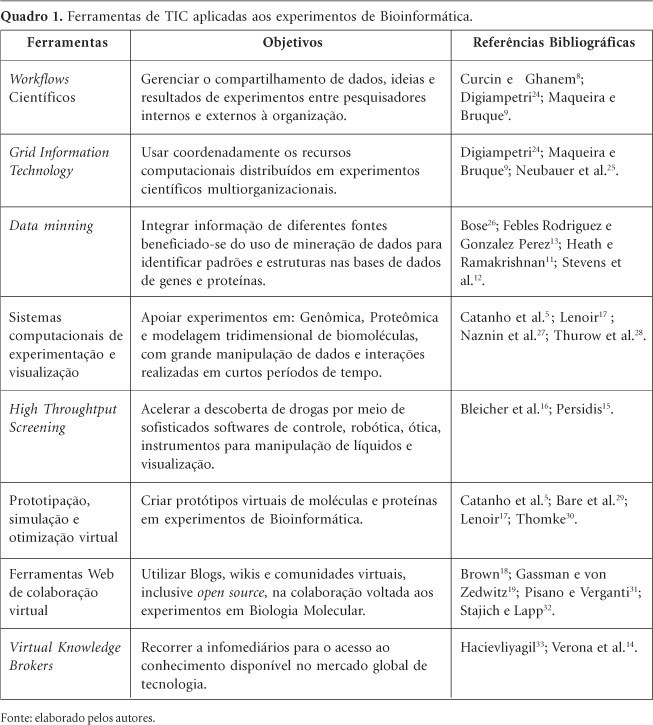
\includegraphics[width=\textwidth]{1413-8123-csc-19-01-00257-gf01}
\caption{}\label{fig:f01}

\end{figure}
\begin{figure}
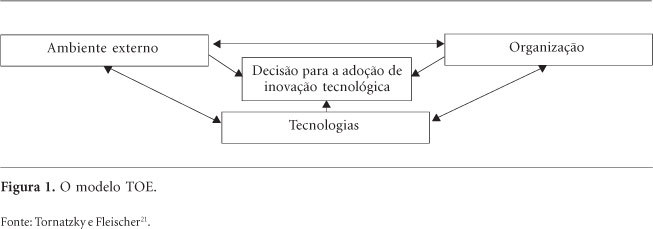
\includegraphics[width=\textwidth]{1413-8123-csc-19-01-00257-gf02}

\caption{}\label{fig:f02}
\end{figure}
\begin{figure}
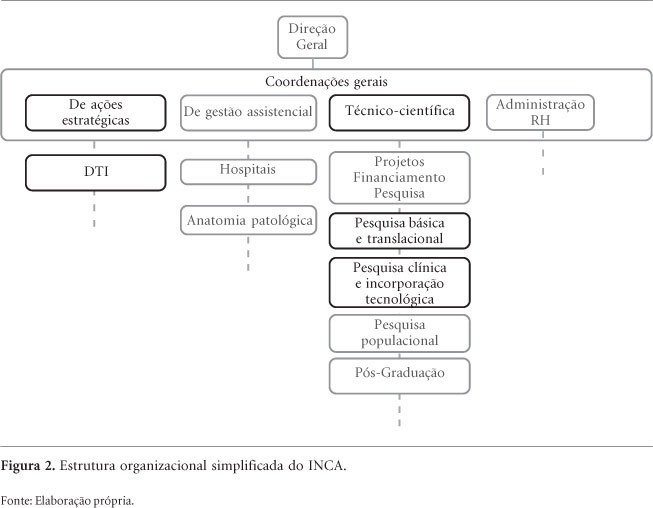
\includegraphics[width=\textwidth]{1413-8123-csc-19-01-00257-gf03}
\caption{}\label{fig:f03}
\end{figure}
\begin{figure}
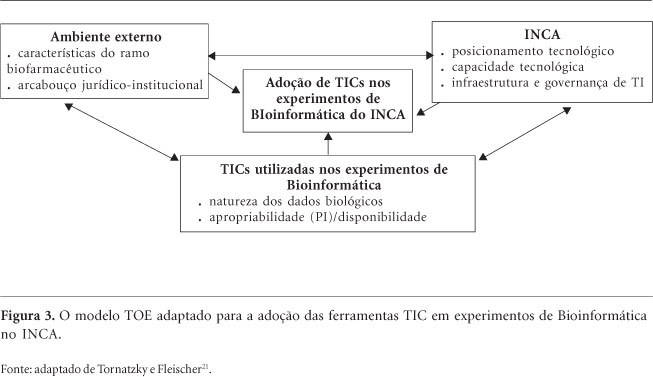
\includegraphics[width=\textwidth]{1413-8123-csc-19-01-00257-gf04}
\caption{}\label{fig:f04}
\end{figure}

\section*{Referências}
\begin{itemize}

\item[1] 1. Macmullen \textsc{wj}, Denn S. Information problems in molecular biology and
Bioinformatics. J of the Amer Soc for Info Sci \& Tech 2005; 56(5):447-456.

\item[2] 2. Attwood \textsc{tk}, Gisel A, Eriksson N-E, Bongcam-Rudloff E. Concepts,
historical milestones and the central place of bioinformatics in modern biology:
a European perspective. In: Mahdavi \textsc{ma}, editor. Bioinformatics-Trends and
Methodologies. Rijeka: Intech Online Publishers; 2011.

\item[3] 3. Costa \textsc{lf}. Bioinformatics: perspectives for the future. Gen Mol Res
2004; 3(4):564-574.

\item[4] 4. Vogt C. Bioinformática, genes e inovação. R ComCiência 2003; 46.

\item[5] 5. Catanho M, De Miranda \textsc{ab}, Degrave W. Comparando genomas: bancos de
dados e ferramentas computacionais para a análise comparativa de genomas
procarióticos. R Eletr de Com Infor \& Inov 2007; 1(2):335-358.

\item[6] 6. Powell W, White D, Koput K, Owen-Smith J. Network Dynamics and field
evolution: the growth of interorganizational collaboration in the life sciences.
\textsc{ajs} 2005; 110(4):1132-1205.

\item[7] 7. Chiaroni D, Chiesa V, Frattini F. Patterns of collaboration along
the Bio-Pharmaceutical innovation process. J of Bus Chem 2008; 5(1):7-22.

\item[8] 8. Curcin V, Ghanem M. Scientific workflow systems - can one size fit
all? Proceedings of the Cairo Biomedical Engineering Conference. Cairo: 2008;
1-9.

\item[9] 9. Maqueira \textsc{jm}, Bruque S. Grid information technology as a new
technological tool for e.science, healthcare and life science. J of Tech Mangt
\& Innov 2007; 2(2):95-113.

\item[10] 10. Critchlow T, Musick R, Slezak T. Experience applying meta-data to
Bioinformatics. Info Sci 2001; 139(1-2):3-17.

\item[11] 11. Heath \textsc{sl}, Ramakrishnan N. The emerging landscape of Bioinformatics
software systems. \textsc{ieee} C 2005; 35(7):41-45.

\item[12] 12. Stevens R, Goble \textsc{ca}, Bechhofer S. Ontology-based knowledge
representation for bioinformatics. B in Bioinf 2000; 1(4):398-414.

\item[13] 13. Febles Rodriguez \textsc{jp}, Gonzalez Perez A. Aplicación de la minería de
datos en la Bioinformática. \textsc{acimed} 2002; 10(2):69-76.

\item[14] 14. Verona G, Prandelli E, Sawhney M. Innovation and virtual
environment: toward virtual knowledge brokers. Org Studies 2006; 27(6):765-788.

\item[15] 15. Persidis A. High-throughput screening. Nat Biotech 1998;
16(5):488-489.

\item[] 16 Bleicher \textsc{kh}, Böhm H-J, Müller K, Alanine \textsc{ai}. Hit and lead generation:
beyond high-throughput screening. Nat R Drug Disc 2003; 2(5):369-378.

\item[17] 17. Lenoir T. Shaping biomedicine as an information science. In:
Bowden \textsc{me}, Hahn \textsc{tb}, Willians \textsc{rv}, editors. Proceedings of the 1998 Conference on
the History and Heritage of Science Information Systems. \textsc{asis} Monograph Series.
Medford: Information Today; 1998. p. 27-45.

\item[18] 18. Brown C. The changing face of scientific discourse: analysis of
Genomic and Proteomic database usage and acceptance, J of the Amer Soct for Info
Sci \& Tech 2003; 54(10):926-938.

\item[19] 19. Gassmann O, von Zedtwitz M. Trends and determinants of managing
virtual R \& D teams. R \& D Mangt 2003; 33(3):243-262.

\item[20] 20. Venkatesh V, Morris \textsc{mg}, Davis \textsc{gb}, Davis \textsc{fd}. User acceptance of
information technology: toward a unified view. \textsc{mis} Quart 2003; 27(3):425-478.

\item[21] 21. Tornatzky \textsc{lg}, Fleischer M. The processes of technological
innovation. Massachusetts: Lexington Books; 1990.

\item[22] 22. Denzin \textsc{nk}, Lincoln \textsc{ys}. Handbook of qualitative research.
California: Sage Publications; 2000.

\item[23] 23. Yin \textsc{rk}. Case study research - design and methods. London: \textsc{sage}
Publications; 1994.

\item[24] 24. Digiampietri \textsc{la}. Gerenciamento de workflows científicos em
Bioinformática [tese]. Campinas: Unicamp; 2007.

\item[25] 25. Neubauer F, Hoheisel A, Geiler J. Workflow-based grid
applications. Fut Gen Comp Syst 2006; 22(1-2):6-15.

\item[26] 26. Bose R. Knowledge management-enabled health care management
systems: capabilities, infrastructure, and decision-support. Exp Syst with
Applic 2003; 24(1):59-71.

\item[27] 27. Naznin F, Sarker R, Essam D. Vertical decomposition with genetic
algorithm for multiple sequence alignment. \textsc{bmc} Bioinf 2011; 12:353-379.

\item[28] 28. Thurow K, Göde B, Dingerdissen U, Stoll N. Laboratory information
management systems for life science applications. Org Proc Res Develop 2004;
8(6): 970-982.

\item[29] 29. Bare \textsc{jc}, Koide T, Reiss \textsc{dj}, Tenenbaum D, Baliga \textsc{ns}. Integration
and visualization of systems biology data in context of the genome. \textsc{bmc} Bioinf
2010; 11:382-390.

\item[30] 30. Thomke \textsc{sh}. Experimentation matters: unlocking the potential of new
technologies for innovation. Boston: \textsc{hbs} Press; 2003.

\item[31] 31. Pisano \textsc{gp}, Verganti R. Which kind of collaboration is right for
you? \textsc{hbr} 2008; 12:78-86.

\item[32] 32. Stajich \textsc{je}, Lapp H. Open source tools and toolkits for
Bioinformatics: significance, and where are we? B in Bioinformatics 2006;
7(3):287-296.

\item[33] 33. Hacievliyagil \textsc{nk}. The impact of open innovation on technology
transfers at Philips and \textsc{dsm} [thesis]. Delft: Delft University of Technology;
2007.

\item[34] 34. Bardin L. Análise de conteúdo. Lisboa: Edições 70; 1979.

\item[35] 35. Malerba F, Orsenigo L. Innovation and market structure in dynamics
of the pharmaceutical industry and Biotechnology: towards a history friendly
model. Ind Corp Change 2001; 11(4):667-703.

\item[36] 36. Chau \textsc{pyk}, Tam \textsc{ky}. Factors affecting the adoption of open systems:
an exploratory study. \textsc{mis} Quart 1997; 21(1):1-24.

\item[37] 37. Pisano \textsc{gp}. Profiting from innovation and the intellectual property
revolution. R Policy 2006; 35:1122-1130.

\item[38] 38. Vieira \textsc{vmm}, Ohayon P. Inovação em fármacos e medicamentos:
estado-da-arte no Brasil e políticas de P \& D. R Econ \& Gestão 2007;
6(13):1-23.

\item[39] 39. Oliveira \textsc{ea}, Labra \textsc{ma}, Bermudez J. A produção pública de
medicamento no Brasil: uma visão geral. Cad Saude Publica 2006;
22(11):2379-2389.

\item[40] 40. Freeman C, Soete L. The economics of industrial innovation.
London: Frances Pinter; 1997.

\item[41] 41. Bell M, Pavitt K. The development of technological capabilities.
In: Haque \textsc{iu}, editor. Trade, technology and international competitiveness.
Washington: World Bank; 1995.

\item[42] 42. Teece D, Pisano G, Shuen A. Dynamic capabilities and strategic
management. Strat Mangt J 1997; 18(7): 509-533.

\item[43] 43. Weill P, Ross \textsc{jw}. \textsc{it} governance. Boston: \textsc{hbs} Press; 2004.

\end{itemize}

\end{document}
